
\documentclass[11pt,letterpaper]{article}

%====================================================================
% 1. MATEMÁTICA Y FUENTES
%====================================================================

% Compilador: XeLaTeX
\usepackage{fontspec}
\usepackage{amsmath}
\usepackage{mathtools}
\usepackage{amsthm}
\usepackage{amssymb}
\usepackage{unicode-math}

%====================================================================
% 2. IDIOMA
%====================================================================

\usepackage{polyglossia}
\setmainlanguage{spanish}

\usepackage{csquotes}
\usepackage{etoolbox}

%====================================================================
% 3. DISEÑO Y FORMATO GENERAL
%====================================================================

\usepackage[margin=1in]{geometry}

\usepackage{microtype}
\usepackage{setspace}
\usepackage{enumitem}
\usepackage{ragged2e}
\usepackage{titlesec}

% Interlineado
\setstretch{1.1}

% Configuración de párrafos
\setlength{\parindent}{1.2em}
\setlength{\parskip}{0pt}
\setlength{\emergencystretch}{2em}

% Configuración de listas
\setlist{
    itemsep=2pt,
    topsep=4pt
}

% Configuración de secciones
\titleformat{\section}
    {\large\bfseries}
    {\thesection}
    {0.6em}
    {}

\titlespacing*{\section}
    {0pt}{1.0ex}{0.5ex}

%====================================================================
% 4. TABLAS
%====================================================================

\usepackage[table]{xcolor}

\usepackage{booktabs}
\usepackage{tabularx}
\usepackage{longtable}
\usepackage{array}

\renewcommand{\arraystretch}{1.02}

%====================================================================
% 5. FIGURAS Y ELEMENTOS GRÁFICOS
%====================================================================

\usepackage{graphicx}
\usepackage{float}
\usepackage{caption}
\usepackage{pdflscape}

\graphicspath{{figuras/}}

% Configuración de títulos de tablas y figuras
\captionsetup{
    font=small,
    labelfont=bf,
    labelsep=period,
    skip=6pt
}

% Espaciado de figuras
\setlength{\textfloatsep}{8pt}
\setlength{\intextsep}{6pt}

%====================================================================
% 6. CÓDIGO Y LISTADOS
%====================================================================

\usepackage{listings}

\lstset{
    language=Python,
    basicstyle=\ttfamily\small,
    frame=lines,
    keywordstyle=\bfseries,
    commentstyle=\itshape\color{gray},
    showstringspaces=false,
    columns=fullflexible,
    xleftmargin=1em
}

%====================================================================
% 7. ENCABEZADOS Y PIES DE PÁGINA
%====================================================================

\usepackage{fancyhdr}

\setlength{\headheight}{15pt}

\pagestyle{fancy}
\fancyhf{}

\renewcommand{\headrulewidth}{0pt}

\fancyhead[R]{
    \small\itshape
    Segunda entrega: diseño y valoración de la cobertura
}

\fancyfoot[C]{
    \small\thepage
}

%====================================================================
% 8. BIBLIOGRAFÍA
%====================================================================

% Procesamiento mediante Biber
\usepackage[
    backend=biber,
    style=ieee,
    sorting=none
]{biblatex}

\addbibresource{references.bib}

%====================================================================
% 9. ENLACES Y REFERENCIAS CRUZADAS
%====================================================================

\usepackage{xurl}

\usepackage[
    colorlinks=true,
    linkcolor=blue!40!black,
    citecolor=blue!40!black,
    urlcolor=blue!40!black,
    pdfusetitle
]{hyperref}

\hypersetup{
    pdftitle={Segunda entrega: diseño y valoración de la cobertura},
    pdfauthor={Anthonny Flores Rojas,
               Andrey Gonzalez Bastos,
               Diego Vega Víquez}
}

\usepackage[capitalise]{cleveref}

% Nombres utilizados en las referencias cruzadas
\crefname{theorem}{Teorema}{Teoremas}
\crefname{proposition}{Proposición}{Proposiciones}
\crefname{lemma}{Lema}{Lemas}
\crefname{corollary}{Corolario}{Corolarios}
\crefname{definition}{Definición}{Definiciones}
\crefname{example}{Ejemplo}{Ejemplos}
\crefname{conjecture}{Conjetura}{Conjeturas}
\crefname{section}{Sección}{Secciones}
\crefname{table}{Tabla}{Tablas}
\crefname{figure}{Figura}{Figuras}
\crefname{equation}{ecuación}{ecuaciones}

%====================================================================
% 10. TEOREMAS Y ENTORNOS MATEMÁTICOS
%====================================================================

\theoremstyle{plain}

\newtheorem{theorem}{Teorema}[section]
\newtheorem{proposition}[theorem]{Proposición}
\newtheorem{lemma}[theorem]{Lema}
\newtheorem{corollary}[theorem]{Corolario}
\newtheorem{conjecture}[theorem]{Conjetura}

\theoremstyle{definition}

\newtheorem{definition}[theorem]{Definición}
\newtheorem{example}[theorem]{Ejemplo}

\theoremstyle{remark}

\newtheorem{remark}[theorem]{Observación}

% Numeración de ecuaciones por sección
\numberwithin{equation}{section}

% Nombre de las demostraciones
\AtBeginDocument{
    \renewcommand{\proofname}{Demostración}
}

%====================================================================
% 11. COMANDOS MATEMÁTICOS
%====================================================================

\newcommand{\R}{\mathbb{R}}
\newcommand{\Z}{\mathbb{Z}}
\newcommand{\E}{\mathbb{E}}

\renewcommand{\P}{\mathbb{P}}

\newcommand{\dd}{\,\mathrm{d}}

\newcommand{\norm}[1]{%
    \lVert #1\rVert
}

\newcommand{\Sh}{\mathcal{S}}

\DeclareMathOperator{\LSE}{LSE}

%====================================================================
% 12. ENTORNOS MATEMÁTICOS EN ESPAÑOL
%====================================================================

\newtheorem{teorema}[theorem]{Teorema}
\newtheorem{proposicion}[theorem]{Proposición}
\newtheorem{lema}[theorem]{Lema}
\newtheorem{corolario}[theorem]{Corolario}
\newtheorem{definicion}[theorem]{Definición}
\newtheorem{ejemplo}[theorem]{Ejemplo}
\newtheorem{observacion}[theorem]{Observación}

%====================================================================
% 13. COMANDOS PARA MONEDAS
%====================================================================

\newcommand{\eur}{\texttt{EUR}\,}
\newcommand{\gbp}{\texttt{GBP}\,}
\newcommand{\czk}{\texttt{CZK}\,}

%====================================================================
% 14. COMANDOS AUXILIARES DEL INFORME
%====================================================================

\newcommand{\estado}[1]{\textbf{#1}}

\newcommand{\sw}{\begin{singlespace}}
\newcommand{\ew}{\end{singlespace}}

\newcommand{\ph}[1]{%
    \textcolor{red!70!black}{\textit{[#1]}}
}

% Porcentajes
\newcommand{\pc}{\mbox{\,\%}}

%====================================================================
% 15. ENTORNO PARA CÓDIGO PYTHON
%====================================================================

\lstdefinestyle{pythonstyle}{
    language=Python,
    basicstyle=\ttfamily\footnotesize,
    keywordstyle=\color{blue!65!black}\bfseries,
    commentstyle=\color{green!35!black}\itshape,
    stringstyle=\color{orange!60!black},
    numberstyle=\tiny\color{gray},
    numbers=left,
    numbersep=10pt,
    stepnumber=1,
    backgroundcolor=\color{gray!5},
    frame=single,
    rulecolor=\color{gray!35},
    framerule=0.4pt,
    framesep=8pt,
    breaklines=true,
    breakatwhitespace=false,
    breakindent=0pt,
    showstringspaces=false,
    keepspaces=true,
    columns=fullflexible,
    tabsize=4,
    captionpos=b,
    aboveskip=12pt,
    belowskip=12pt
}

\lstnewenvironment{pythoncode}[1][]%
    {\lstset{style=pythonstyle,#1}}%
    {}

%====================================================================
% 16. DATOS INSTITUCIONALES
%====================================================================

\newcommand{\Universidad}{Universidad de Costa Rica}
\newcommand{\Escuela}{Escuela de Matemáticas}

\newcommand{\Curso}{
    Valoración de instrumentos financieros (CA0308)
}

\newcommand{\Profesor}{
    Daniel Vargas Carrillo
}

%====================================================================
% 17. DATOS DEL DOCUMENTO
%====================================================================

\title{
    \textbf{Diseño y valoración de una cobertura con opciones para ČEZ}\\[0.4em]
    \large Segunda entrega: diseño y valoración de la cobertura
}

\author{%
    {Anthonny Flores Rojas}
    \thanks{
        Escuela de Matemáticas,
        Universidad de Costa Rica.
        \texttt{anthonny.flores@ucr.ac.cr}
    }
    \and
    {Andrey Gonzalez Bastos}
    \thanks{
        Escuela de Matemáticas,
        Universidad de Costa Rica.
        \texttt{andrey.gonzalezbastos@ucr.ac.cr}
    }
    \and
    {Diego Vega Víquez}
    \thanks{
        Escuela de Matemáticas,
        Universidad de Costa Rica.
        \texttt{diego.vega@ucr.ac.cr}
    }
}

\date{
    Curso: Valoración de instrumentos financieros (CA0308)\\
    Profesor: Daniel Vargas Carrillo\\[0.3em]
    \today
}

%====================================================================
% INICIO DEL DOCUMENTO
%====================================================================

\begin{document}

\maketitle

\tableofcontents

\newpage

\section{Introducción y continuidad con la primera entrega}

La primera entrega descompuso la posición de ČEZ, a.~s., en cuatro capas: una capa física larga (45,5~TWh de generación esperada para 2023), una capa financiera corta (22,3~TWh vendidos a plazo a EUR~54,3/MWh \cite{cez_q3_2021}), una capa económica neta larga (23,2~TWh sin vender) y una capa de liquidez corta ante alzas, porque las ventas a plazo pierden valor cuando el precio sube y, si están sujetas a garantías, exigen efectivo antes de que se cobre la producción. Este último es el mecanismo que Giannozzi y Kirilova \cite{GIANNOZZI2026107700} documentan para las energéticas europeas; se utiliza aquí como fundamento conceptual y no como información disponible en la fecha de decisión.

Este informe responde qué instrumento se habría utilizado, por cuánto, a qué precio y por qué. Todas las cifras provienen del Excel auditable de la entrega (se indica la hoja entre paréntesis) y emplean únicamente datos anteriores al 23 de febrero de 2022: el futuro anual de electricidad base alemana para 2023 (Cal-23) cotizaba a EUR~156,43/MWh \cite{energycharts_futuros_de}, el tipo de cambio era de CZK~24,475 por euro \cite{cnbfx} y la liquidez de referencia, efectivo más líneas comprometidas no dispuestas al 30 de septiembre de 2021, ascendía a CZK~39.423 millones \cite{cez_interim_q3_2021,cez_q3_2021}. Las primas, los márgenes y las holguras de liquidez son estimaciones propias y se presentan como tales.

\section{Selección y comparación de instrumentos}

Se comparan dos opciones europeas compradas sobre el Cal-23. Cada una responde a una capa distinta, y esa es la base de la elección. La \emph{call} otorga el derecho a comprar el futuro al precio de ejercicio $K$ y paga cuando el precio sube, que es el escenario en que la capa financiera corta pierde valor y la capa de liquidez exige efectivo. La \emph{put} otorga el derecho a vender a $K$ y paga cuando el precio baja: protegería el ingreso de la capa económica larga residual, pero no aporta nada en un alza. La Tabla~\ref{tab:comp} resume la comparación e incorpora los futuros como referencia.

\begin{table}[H]
    \centering\small
    \caption{Comparación de instrumentos (hoja \textsc{comparacion}).}\label{tab:comp}
    \begin{tabular}{@{}p{2.7cm}p{4.1cm}p{4.1cm}p{4.2cm}@{}}
        \toprule
            Criterio & Call comprada (elegida) & Put comprada & Futuros (referencia)\\
        \midrule
            Capa que protege & Financiera corta; liquidez ante alzas & Económica neta larga & Vendido: capa larga. Comprado: deshace la venta\\
            Paga si el precio & Sube sobre $K$ & Baja bajo $K$ & Simétrico\\
            Costo inicial & Prima & Prima (igual con $K=F$, $r=0$) & Sin prima; margen inicial\\
            Pérdida máxima & La prima & La prima & Ilimitada\\
            Garantías & Ninguna tras la prima (estilo prima) & Ninguna tras la prima & Margen inicial y de variación diario\\
            Caja ante un alza & No agrega salidas; compensa al vencimiento & No agrega salidas ni compensa & Vendido: nuevas llamadas de margen\\
        \bottomrule
    \end{tabular}
\end{table}

Con $K=F$ y $r=0$ ambas opciones cuestan lo mismo por MWh (Sección~\ref{sec:val}), de modo que la elección no depende del precio sino del riesgo que se prioriza. Se elige la call porque el riesgo central identificado es de liquidez y proviene de las posiciones cortas existentes: ante un alza de 30\pc{}, las ventas de 2023 pierden EUR~1.046,5 millones de valor, y la call, sobre ese mismo volumen, paga exactamente esa cifra al vencimiento, mientras que la put vence sin valor (hoja \textsc{comparacion}). La put, en cambio, cubriría una caída que no genera llamadas de margen sobre las ventas existentes.

Dos precisiones acotan el argumento. Primero, la call compensa el \emph{resultado económico}, no el calendario de caja: no elimina las llamadas de margen. Que su valor esté disponible para atenderlas depende del régimen de liquidación (si la opción se liquida a diario como un futuro o solo paga la prima al inicio \cite{eccm,ecc46}), de que pueda venderse antes del vencimiento y de la oportunidad de los flujos. Segundo, ČEZ es larga neta, por lo que la call no reduce su riesgo económico total: es una cobertura de la capa corta. Los futuros se descartan por el canal de liquidez: vender futuros sobre 6,69~TWh exigiría, con el margen de referencia de 17,1\pc{} del nocional, EUR~179 millones de margen inicial y EUR~314 millones de margen de variación ante un alza de 30\pc{} (hoja \textsc{liquidez}), es decir, agravaría la presión sobre la caja; comprarlos equivaldría a deshacer la venta y cristalizar una pérdida de EUR~2.277 millones (hoja \textsc{exposicion}).

\section{Valoración de las opciones mediante Black-76}\label{sec:val}

Las opciones europeas sobre futuros se valoran con el modelo de Black \cite{black}:
\begin{equation}
C=e^{-rT}\left[F\,N(d_1)-K\,N(d_2)\right],\qquad
P=e^{-rT}\left[K\,N(-d_2)-F\,N(-d_1)\right],\label{eq:b76}
\end{equation}
\begin{equation*}
d_1=\frac{\ln(F/K)+\tfrac{1}{2}\sigma^{2}T}{\sigma\sqrt{T}},\qquad d_2=d_1-\sigma\sqrt{T},
\end{equation*}
donde $F$ es el precio del futuro, $K$ el precio de ejercicio, $T$ el tiempo al vencimiento en años, $r$ la tasa de descuento, $\sigma$ la volatilidad anual y $N(\cdot)$ la distribución normal estándar acumulada. Los parámetros son $F=K=156{,}43$~EUR/MWh (strike ATM), $T=0{,}8$ años y $r=0$, coherente con la tasa de política del BCE en el corte. La volatilidad principal es la histórica anualizada del Cal-23 con todo el historial disponible (295 rendimientos logarítmicos diarios, 41,24\pc{}); las ventanas de 126 y 60 días (57,18\pc{} y 72,39\pc{}) se usan como sensibilidad, porque la volatilidad casi se duplica al acortar la ventana (hoja \textsc{datos\_mercado}).


\begin{table}[H]
    \centering\small
    \caption{Primas Black-76 de la call y la put ATM
    (hoja \textsc{black76}).}
    \label{tab:primas}
    \begin{tabular}{@{}lccc@{}}
        \toprule
        & $\sigma$ principal & $\sigma$ 126 días & $\sigma$ 60 días\\
        \midrule
        Volatilidad anual & 41,24\pc{} & 57,18\pc{} & 72,39\pc{}\\
        $d_1=-d_2$ & 0,1844 & 0,2557 & 0,3238\\
        Prima de la call (EUR/MWh) & 22,89 & 31,57 & 39,71\\
        Prima de la put (EUR/MWh) & 22,89 & 31,57 & 39,71\\
        Prima / $F$ & 14,6\pc{} & 20,2\pc{} & 25,4\pc{}\\
        Punto de equilibrio de la call (EUR/MWh)
            & 179,32 & 188,00 & 196,14\\
        \bottomrule
    \end{tabular}

    \par\vspace{3pt}
    \begin{minipage}{0.95\linewidth}
        \footnotesize
        \textit{Nota:} Las primas unitarias se expresan en EUR/MWh.
    \end{minipage}
\end{table}


La igualdad de primas es la paridad put-call, $C-P=e^{-rT}(F-K)=0$, que el Excel emplea como control de valoración. Las primas son estimaciones teóricas con volatilidad histórica, no cotizaciones observadas de EEX: no se dispuso de precios de liquidación ni de volatilidad implícita de las opciones al corte. La incertidumbre es material, pues cada punto porcentual de volatilidad mueve la prima unos EUR~0,55/MWh y el rango entre estimadores va de EUR~22,89 a 39,71/MWh.

\section{Diseño y elección del nivel de cobertura}

La base de la cobertura es la capa financiera corta de 2023 (22,3~TWh), que es el volumen que la call protege. El \emph{nivel de cobertura} es la fracción de esa base que se cubre (30\pc{}, 70\pc{} o 100\pc{}); la \emph{razón de cobertura} $h$ es la cantidad de MWh de opción por MWh expuesto, y se fija en $h=1$ porque la opción y las ventas a plazo comparten subyacente. El volumen es base $\times$ nivel $\times\,h$, y cada contrato equivale a 1~MW durante las 8.760 horas de 2023 \cite{eex}.

\begin{table}[H]
    \centering\small
    \caption{Niveles de cobertura con la call ATM y la volatilidad principal (hojas \textsc{cobertura} y \textsc{liquidez}).}\label{tab:niveles}
    \begin{tabular}{@{}lrrr@{}}
    \toprule
        & 30\pc{} & 70\pc{} & 100\pc{}\\
    \midrule
        Volumen cubierto (TWh) & 6,69 & 15,61 & 22,30\\
        Contratos operables & 764 & 1.782 & 2.546\\
        Nocional (EUR mill.) & 1.046,5 & 2.441,9 & 3.488,4\\
        Prima total (EUR mill.) & 153,1 & 357,3 & 510,4\\
        Prima total (CZK mill.) & 3.747 & 8.744 & 12.492\\
        Prima / liquidez de referencia & 9,5\pc{} & 22,2\pc{} & 31,7\pc{}\\
        Pago ante $+30\pc{}$ / pérdida de la capa corta 2023 & 30\pc{} & 70\pc{} & 100\pc{}\\
        Holgura de liquidez ante $+30\pc{}$ (CZK mil mill.) & 1,86 & $-3{,}14$ & $-6{,}89$\\
    \bottomrule
    \end{tabular}
\end{table}

El criterio de decisión es el costo fijo inicial de la prima y su efecto sobre la liquidez. La prueba es la siguiente: ante un alza de 30\pc{}, si todas las ventas de 2023 y 2024 exigen garantías en efectivo ($\theta=100\pc{}$), el margen de variación heredado consume CZK~33,82 mil millones y deja una holgura de CZK~5,60 mil millones sobre la liquidez de referencia. La prima se paga al inicio y reduce esa holgura en su totalidad. Con el nivel de 30\pc{} la holgura sigue siendo positiva (CZK~1,86 mil millones); con 70\pc{} y 100\pc{} se vuelve negativa. Dicho de otro modo, la holgura financia como máximo una prima equivalente al 45\pc{} de la base ($5{,}60/12{,}49$), de modo que, entre los tres niveles evaluados, solo el de 30\pc{} es compatible con la liquidez en el escenario de estrés.

Aumentar la protección tiene un beneficio claro y un costo proporcional: cada diez puntos adicionales de cobertura compensan EUR~104,7 millones más de pérdida de la capa corta ante un alza de 30\pc{}, pero cuestan EUR~51,0 millones (CZK~1.249 millones) de prima cierta. El nivel de 100\pc{} neutraliza por completo la pérdida de valoración de las ventas de 2023 por encima de $K$, a cambio de comprometer casi un tercio de la liquidez antes de que ocurra movimiento alguno. Se recomienda, por tanto, el nivel de 30\pc{}: 6,69~TWh, 764 contratos y una prima de EUR~153,1 millones (CZK~3.747 millones). La recomendación es sensible a la volatilidad: con la ventana de 126 días la prima sube a EUR~211,2 millones y la holgura cae a CZK~0,43 mil millones; con la de 60 días (EUR~265,7 millones) sería negativa en CZK~0,90 mil millones.

\section{Costo, liquidez, escenarios y recomendación}

%\textbf{Punto de equilibrio.} 
El resultado neto por MWh de la call comprada es
\begin{equation}
\pi(F_T)=\max(F_T-K,\,0)-c,\label{eq:neto}
\end{equation}
con $c$ la prima. Se distinguen dos umbrales. La call tiene pago positivo cuando $F_T>K=156{,}43$; produce ganancia neta solo cuando $F_T>K+c=156{,}43+22{,}89=179{,}32$~EUR/MWh, es decir, tras un alza de 14,6\pc{} respecto del precio inicial (hoja \textsc{escenarios}). Por debajo del strike se pierde toda la prima; entre el strike y el punto de equilibrio el pago recupera parte de ella; por encima, la opción gana un euro por cada euro de alza. Con las volatilidades de sensibilidad el umbral sube a EUR~188,00 y 196,14/MWh ($+20{,}2\pc{}$ y $+25{,}4\pc{}$). Este es el equilibrio de la opción aislada, no el de la empresa: el resultado económico conjunto de 2023, $Q_TF_T+Q_h(K_s-F_T)+N\,\pi(F_T)$, con $Q_T=45{,}5$~TWh, $Q_h=22{,}3$~TWh, $K_s=54{,}3$ y $N$ el volumen cubierto, es positivo y creciente en todos los escenarios; la call lo reduce en el monto de la prima cuando el precio no supera el umbral y lo eleva por encima de él.

\begin{table}[H]
    \centering\small
    \caption{Resultados por escenario con el nivel de 30\pc{} (EUR millones; hojas \textsc{escenarios} y \textsc{liquidez}).}\label{tab:esc}
    \begin{tabular}{@{}rrrrrrrr@{}}
    \toprule
        Variación & Precio & Capa corta & Call neta & Put neta & \multicolumn{3}{c}{Resultado económico 2023}\\
    \cmidrule(l){6-8}
        del precio & (EUR/MWh) & (cambio de valor) & de prima & de prima & Sin cobertura & Con call & Con put\\
    \midrule
        $-30\pc{}$ & 109,50 & $+1.046{,}5$ & $-153{,}1$ & $+160{,}8$ & 3.751,3 & 3.598,2 & 3.912,2\\
        $-20\pc{}$ & 125,14 & $+697{,}7$ & $-153{,}1$ & $+56{,}2$ & 4.114,2 & 3.961,1 & 4.170,4\\
        $-10\pc{}$ & 140,79 & $+348{,}8$ & $-153{,}1$ & $-48{,}5$ & 4.477,1 & 4.324,0 & 4.428,7\\
        $0\pc{}$ & 156,43 & 0,0 & $-153{,}1$ & $-153{,}1$ & 4.840,1 & 4.687,0 & 4.687,0\\
        $+10\pc{}$ & 172,07 & $-348{,}8$ & $-48{,}5$ & $-153{,}1$ & 5.203,0 & 5.154,5 & 5.049,9\\
        $+20\pc{}$ & 187,72 & $-697{,}7$ & $+56{,}2$ & $-153{,}1$ & 5.565,9 & 5.622,1 & 5.412,8\\
        $+30\pc{}$ & 203,36 & $-1.046{,}5$ & $+160{,}8$ & $-153{,}1$ & 5.928,8 & 6.089,7 & 5.775,7\\
    \bottomrule
    \end{tabular}
\end{table}

% \textbf{Escenarios.} 
La Tabla~\ref{tab:esc} muestra que la call y la put son imágenes especulares. Ante un alza de 30\pc{} la call de 30\pc{} paga EUR~314,0 millones, que compensan el 30\pc{} de la pérdida de la capa corta y dejan una ganancia neta de EUR~160,8 millones; la put pierde su prima. Si el precio no sube, el costo de la protección es la prima completa (EUR~153,1 millones, 3,2\pc{} del resultado económico de 2023 sin cobertura). Con el nivel de 100\pc{} la pérdida de la capa corta quedaría acotada en EUR~510,4 millones, la prima, para cualquier alza.

% \textbf{Costo, garantías y liquidez.} 
Conviene separar tres conceptos que el Excel calcula por separado. La \emph{prima} es el único desembolso del comprador en el régimen estilo prima: CZK~3.747 millones al inicio, más unos CZK~135 millones de costo financiero hasta el vencimiento a la tasa repo de 4,50\pc{} \cite{cnb_2022} y EUR~16.725 de comisión de compensación; no se le atribuye margen inicial ni de variación, aunque el régimen vigente al corte no pudo verificarse. La \emph{ganancia económica} (EUR~160,8 millones ante $+30\pc{}$) se cobra al vencimiento. El \emph{efectivo disponible para garantías} durante la vida de la opción es nulo en ese régimen: la revalorización de la call tras un choque instantáneo de 30\pc{} (EUR~221,9 millones) solo se convierte en caja si la opción se vende o si se liquida a diario. Las llamadas de margen de las posiciones existentes subsisten íntegras: ante $+30\pc{}$ ascienden a EUR~1.381,8 millones para 2023 y 2024 con $\theta=100\pc{}$, y el pago de la call al vencimiento equivale al 22,7\pc{} de esa cifra. La pérdida económica y la salida de efectivo no coinciden ni en monto ni en fecha.

Los resultados dependen de tres supuestos no observados. Con $\theta=50\pc{}$ la holgura con la call asciende a CZK~18,8 mil millones y los tres niveles serían financiables; si se añaden las ventas de 2022 pendientes de entrega (valoradas con el Cal-23 como cota inferior), la liquidez de referencia es insuficiente con $\theta=100\pc{}$ incluso sin nueva cobertura (CZK~$-30{,}9$ mil millones). El margen de 17,1\pc{} procede de un aviso de CME para el futuro mensual de electricidad alemana \cite{cme}: es una referencia fechada, no un margen histórico verificado de ECC. Y la liquidez es la de septiembre de 2021.

% \textbf{Recomendación.} 
Se habría comprado una \emph{call europea ATM sobre el futuro Cal-23} ($K=156{,}43$~EUR/MWh, vencimiento supuesto en diciembre de 2022) para proteger la capa financiera corta de 2023, con un nivel de cobertura de 30\pc{} de sus 22,3~TWh: 6,69~TWh, 764 contratos, a una prima estimada de EUR~22,89/MWh, es decir, EUR~153,1 millones (CZK~3.747 millones, 9,5\pc{} de la liquidez de referencia). La opción genera ganancias netas a partir de EUR~179,32/MWh. Se prefiere a la put porque el riesgo priorizado es el que describen Giannozzi y Kirilova \cite{GIANNOZZI2026107700}: una cobertura económicamente razonable que drena liquidez cuando el precio sube. La call es el único de los instrumentos comparados que paga en ese escenario sin crear nuevas llamadas de margen, y el nivel de 30\pc{} es el único de los tres que conserva holgura de liquidez en el estrés. Sus límites son tres: la prima es teórica y la recomendación no resiste la volatilidad de 60 días; la call compensa al vencimiento y no elimina las llamadas de margen; y aumenta la exposición neta al alza de una empresa que ya es larga, por lo que deja sin protección la caída del precio de la generación no vendida.

\clearpage
  \printbibliography[title={Referencias bibliográficas}]



\clearpage
\appendix

\section*{Anexos}
\addcontentsline{toc}{section}{Anexos}
\renewcommand{\thefigure}{A\arabic{figure}}
\renewcommand{\thetable}{A\arabic{table}}
\setcounter{figure}{0}
\setcounter{table}{0}

\subsection*{A. Diagramas de pagos}

\begin{figure}[H]
\centering
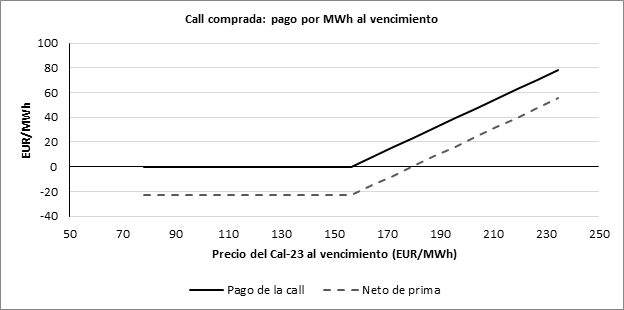
\includegraphics[width=0.495\textwidth]{images/grafico_1.png}\hfill
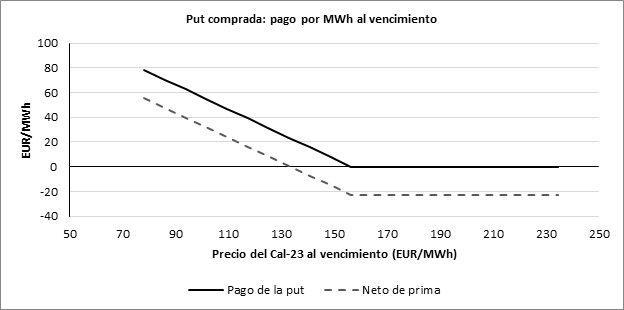
\includegraphics[width=0.495\textwidth]{images/grafico_2.png}
\caption{Pago por MWh al vencimiento de la call y de la put compradas ($K=156{,}43$; prima de EUR~22,89/MWh con la volatilidad principal). Fuente: Excel auditable, hoja \textsc{graficos}.}\label{fig:pagos}
\end{figure}

\subsection*{B. Resultados por escenario}

\begin{figure}[H]
\centering
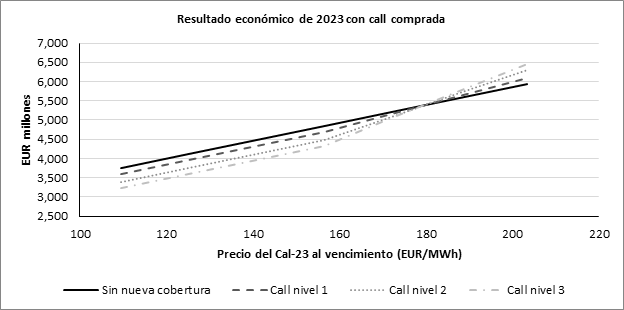
\includegraphics[width=0.495\textwidth]{images/grafico_3.png}\hfill
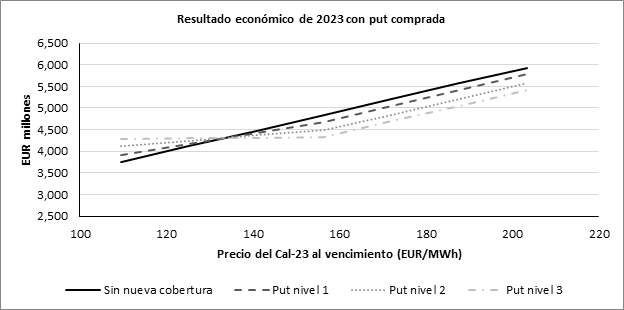
\includegraphics[width=0.495\textwidth]{images/grafico_4.png}
\caption{Resultado económico de 2023 (ingreso físico, ventas a plazo y opción) por nivel de cobertura. Niveles 1, 2 y 3: 30\pc{}, 70\pc{} y 100\pc{} de 22,3~TWh. Fuente: Excel auditable, hoja \textsc{graficos}.}\label{fig:result}
\end{figure}

\subsection*{C. Liquidez}

\begin{figure}[H]
\centering
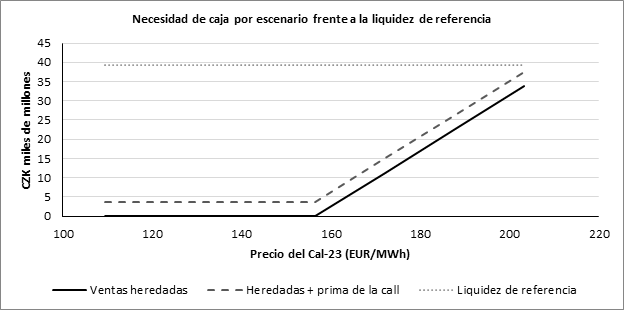
\includegraphics[width=0.495\textwidth]{images/grafico_5.png}\hfill
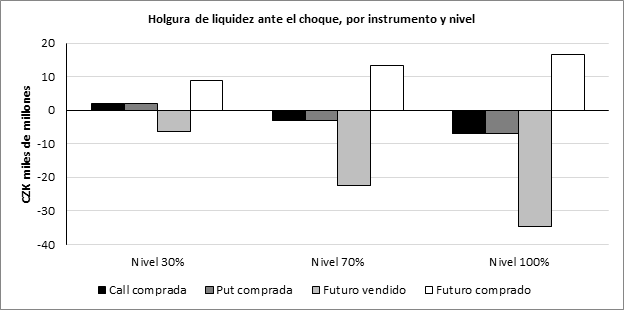
\includegraphics[width=0.495\textwidth]{images/grafico_6.png}
\caption{Izquierda: necesidad de caja por escenario frente a la liquidez de referencia (ventas de 2023 y 2024, $\theta=100\pc{}$, call al 30\pc{}). Derecha: holgura de liquidez ante un alza de 30\pc{} por instrumento y nivel; los futuros usan el margen de referencia de CME, que no equivale al de ECC. Fuente: Excel auditable, hoja \textsc{graficos}.}\label{fig:liq}
\end{figure}

\subsection*{D. Tablas complementarias}

\begin{table}[H]
\centering\small
\caption{Holgura de liquidez ante un alza de 30\pc{} (CZK miles de millones; hoja \textsc{liquidez}). Liquidez de referencia: 39,42.}\label{tab:holgura}
\begin{tabular}{@{}lrrrrrrrr@{}}
\toprule
Ventas heredadas & $\theta$ & Consumo & Sin nueva & \multicolumn{3}{c}{Call o put comprada} & \multicolumn{2}{c}{Futuro vendido}\\
\cmidrule(lr){5-7}\cmidrule(l){8-9}
incluidas & & heredado & cobertura & 30\pc{} & 70\pc{} & 100\pc{} & 30\pc{} & 100\pc{}\\
\midrule
2023 & 100\pc{} & 25,61 & 13,81 & 10,06 & 5,07 & 1,32 & 1,74 & $-26{,}44$\\
2023 y 2024 & 100\pc{} & 33,82 & 5,60 & 1,86 & $-3{,}14$ & $-6{,}89$ & $-6{,}47$ & $-34{,}64$\\
2023 y 2024 & 50\pc{} & 16,91 & 22,51 & 18,77 & 13,77 & 10,02 & 10,44 & $-17{,}73$\\
2023, 2024 y 2022 & 100\pc{} & 70,32 & $-30{,}90$ & $-34{,}65$ & $-39{,}64$ & $-43{,}39$ & $-42{,}97$ & $-71{,}15$\\
2023, 2024 y 2022 & 50\pc{} & 35,16 & 4,26 & 0,51 & $-4{,}48$ & $-8{,}23$ & $-7{,}81$ & $-35{,}98$\\
\bottomrule
\end{tabular}
\end{table}

\begin{table}[H]
\centering\small
\caption{Prima total de la call sobre la capa corta por volatilidad y nivel (EUR millones; hoja \textsc{matrices\_valoracion}).}\label{tab:matriz}
\begin{tabular}{@{}lrrr@{}}
\toprule
Nivel de cobertura & $\sigma=41{,}24\pc{}$ & $\sigma=57{,}18\pc{}$ & $\sigma=72{,}39\pc{}$\\
\midrule
30\pc{} (6,69 TWh) & 153,1 & 211,2 & 265,7\\
70\pc{} (15,61 TWh) & 357,3 & 492,9 & 619,9\\
100\pc{} (22,30 TWh) & 510,4 & 704,1 & 885,6\\
\bottomrule
\end{tabular}
\end{table}

\begin{table}[H]
\centering\small
\caption{Sensibilidad de la prima de la call al strike y al vencimiento (EUR/MWh; hoja \textsc{black76}).}\label{tab:sens}
\begin{tabular}{@{}lrrr@{\hspace{1.2cm}}lrrr@{}}
\toprule
$K/F$ & 41,24\pc{} & 57,18\pc{} & 72,39\pc{} & $T$ (años) & 41,24\pc{} & 57,18\pc{} & 72,39\pc{}\\
\midrule
90\pc{} & 30,43 & 38,44 & 46,03 & 0,25 & 12,84 & 17,78 & 22,47\\
100\pc{} & 22,89 & 31,57 & 39,71 & 0,50 & 18,13 & 25,06 & 31,60\\
110\pc{} & 17,00 & 25,89 & 34,31 & 0,80 & 22,89 & 31,57 & 39,71\\
120\pc{} & 12,50 & 21,22 & 29,70 & 1,00 & 25,55 & 35,21 & 44,21\\
\bottomrule
\end{tabular}
\end{table}

\begin{table}[H]
\centering\small
\caption{Clasificación de la información utilizada.}\label{tab:clas}
\begin{tabular}{@{}p{3.2cm}p{12.3cm}@{}}
\toprule
Categoría & Elementos\\
\midrule
Observado & Precio del Cal-23 y del Cal-24 al corte; ventas a plazo de 2022 a 2024 (volúmenes y precios); efectivo y líneas de crédito al 30-sep-2021; tipo de cambio; tasa repo; aviso de margen de CME.\\
Estimación propia & Volatilidad histórica; primas Black-76; contratos, nocionales y primas totales; margen de 17,1\pc{} del nocional; resultados por escenario y holguras de liquidez.\\
Supuesto o pendiente & $T=0{,}8$ años y $r=0$; $\theta$; régimen de liquidación de la opción; margen de ECC; precios de mercado de 2022; liquidez y porcentaje vendido en febrero de 2022; cotizaciones de opciones de EEX.\\
\bottomrule
\end{tabular}
\end{table}



\end{document}
